% Options for packages loaded elsewhere
\PassOptionsToPackage{unicode}{hyperref}
\PassOptionsToPackage{hyphens}{url}
%
\documentclass[11pt]{ctexart}
\usepackage[vmargin=1.5cm,  hmargin=2.5cm]{geometry}

\usepackage{amssymb, amsmath}
\usepackage{xcolor}
\usepackage{hyperref}
\hypersetup{hidelinks}
\urlstyle{same} % disable monospaced font for URLs
\usepackage{graphicx}

%%%%%%%%%% SET CJK FONT
\usepackage{fourier}
\setCJKmainfont[ItalicFont=Adobe Kaiti Std,  SmallCapsFont=*]{Noto Sans CJK SC}
\setCJKsansfont{Noto Sans CJK SC}
\setCJKmonofont{Noto Sans Mono CJK SC}
%%%%%%%%%%%%%%%%%%%%%%%%%%

%%%%%%%%%%%%%%%%%%%%%%%%%%%%%%%%%%%%%
\usepackage{fancyhdr}
\pagestyle{fancy} 
\fancyhead[L]{\textit{《宏观经济学》}}
\fancyhead[C]{\texttt{第} \thepage \textit{页}}
\fancyhead[R]{\textit{数字经济专业}}
\fancyfoot[L]{\textit{湖南大学课程}}
\fancyfoot[R]{\thepage}
\fancyfoot[C]{\textit{授课教师:雷浩然}}
%%%%%%%%%%%%%%%%%%%%%%%%%%%%%%%%%%%%%

\author{}
\date{}

\begin{document}
\begin{center}
  \subsection*{IS-LM: 产品市场和货币市场的短期均衡}
\end{center}

\paragraph{产品市场与 IS 曲线}
\begin{itemize}
\item
  凯恩斯交叉模型的均衡条件: \textbf{计划投资}等于\textbf{实际投资}. 其中计划投资 $\bar{I}$ 的值是外生给定的.
\item
  实际生活中,  投资需求取决于融资成本,  影响融资成本的核心变量是(借贷)利率 $r$.

  \begin{itemize}
  \item
    投资函数:$I(r)$. 它是减函数, 对应的投资曲线向下倾斜,  见图1(a).
  \item 
    考虑利率时,  凯恩斯交叉的均衡方程变为下方 (IS) 方程,  均衡时 $Y$ 与 $r$ 负相关:
    \begin{equation*}
      Y = C(Y) + I(r) + G. 
      \tag{IS}  
    \end{equation*}
 
  \item
    画图推导 IS 曲线:(a)利率提高导致计划投资下降
    (b)投资支出下降导致计划支出下降, 从而使均衡产出下降
    (c)综合前两者, 利率提高导致均衡产出下降
  \end{itemize}
\end{itemize}

\begin{figure}[htbp]
\centering
\includegraphics[width=0.8\textwidth]{~/Downloads/is-curve.jpeg}
\caption{画图推导 IS 曲线}
\label{fig:is}
\end{figure}

由于方程(IS)包含两个内生变量,  我们还需要考虑货币市场的均衡才能确定均衡时的总产出$Y$和利率$r$.

IS-LM 模型名称的由来: IS = ``\textbf{I}nvestment and \textbf{S}avings",  LM = ``\textbf{L}iquidity and \textbf{M}oney supply''

\paragraph{流动性偏好 (Liquidity preference)}
\begin{itemize}
\item
  IS 曲线中利率是外生给定的,  我们无法得知利率是如何决定的.
\item
  凯恩斯在《通论》一书中提出\textbf{流动性偏好}理论.
\item
  之所以叫流动性偏好, 是因为这个理论分析的是货币市场, 而\textbf{流动性}是人们愿意``持有货币''而非``持有其它资产''的原因. 这里的其它资产包括实体资产和除了货币以外的金融资产.
\end{itemize}

\paragraph{实际货币余额供给}

\begin{itemize}
\item
  记名义货币供给为 $M$,  价格水平为 $P$,  则实际货币余额供给为 $M/P$.
\item
  假设实际货币余额的\textbf{供给}是外生给定的: $(M/P)^s = \bar{M}/ \bar{P}$
  \begin{itemize}
  \item
    假设的理由: 名义货币供给 $\bar{M}$ 由央行决定,  价格水平 $\bar{P}$ 在短期固定不变
  \end{itemize}
\end{itemize}

\paragraph{实际货币余额需求 (流动性偏好理论)}

\begin{itemize}
\item
  实际货币余额需求由利率和产出决定:$(M/P)^d = L(Y,  r)$, $L$ 为居民对实际货币余额的需求函数.
\item
  $L$ 关于 $r$ 递减, 因为利率是持有货币的机会成本. 这里的利率应理解为回报率, 比如购买债券的投资回报率.
  \begin{itemize}
  \item
    张三月入一万,  他考虑将财富在两种资产(货币和债券)上进行分配:
  \item
    货币流动性高, 可直接用于交易; 但货币不能生息.
  \item
    债券的收益率为 $r$,  但流动性差,  一般不能直接用于购买商品.
  \item
    当利率上升时, 张三愿意牺牲更多的流动性 (即持有更少货币),  以换取高投资回报. 因此, 张三的货币需求和利率负相关. 
  \end{itemize}
\end{itemize}

均衡利率由实际货币余额的供给和需求决定, 见图~2. 图~2固定了收入 $Y$,  只考虑 $r$ 对实际货币余额需求的影响.

\begin{center}
\begin{figure}[htbp]
\centering
\includegraphics[width = 0.6\textwidth]{~/Downloads/money-demand.jpeg}
\caption{\centering 固定收入$Y$时, 货币市场的均衡利率 $r$. }
\end{figure}  
\end{center}

\clearpage

实际货币余额需求 $L$ 和 $Y$ 正相关:
\begin{itemize}
\item
  收入上升时, 张三的日常开支也变高, 需要持有更多的货币以便交易.
\end{itemize}
小结: 实际货币余额需求可表示为 $(M/P)^d = L(Y,  r)$, 它与 $Y$ 正相关, 与 $r$ 负相关

\paragraph{LM 曲线}
画图推导 LM 曲线:

\begin{itemize}
\item
  收入上升导致实际货币余额的需求上升, 从而使利率上升: 图3a
\item
  因此,  货币市场的均衡利率与收入 $Y$ 正相关: 图3b
\end{itemize}

\begin{figure}[htbp]
\centering
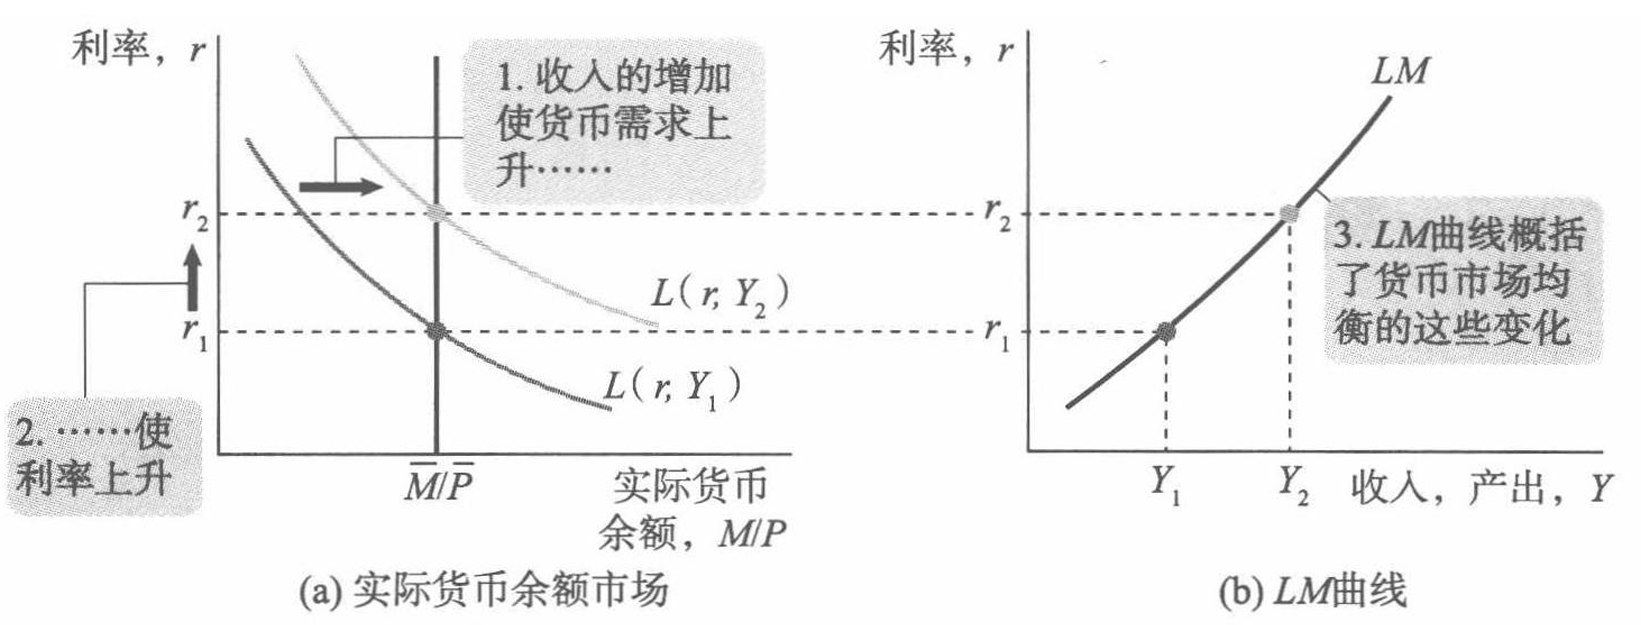
\includegraphics[width=0.9\textwidth]{~/Dropbox/hnu-macro-2021/IMG_0717.jpg}
\caption{根据流动性偏好理论画图推导 LM 曲线}
\end{figure}

\paragraph{IS--LM 模型}

\[Y = C(Y-T) + I(r) + G \tag{IS}\]
\[{\overline{M} / \overline{P}} = L(r, Y) \tag{LM}\]
\begin{itemize}
\item
  IS 曲线表示产品市场的均衡,  均衡条件是``计划投资等于储蓄''. 
\item
  LM 曲线表示货币市场的均衡,  均衡条件是``实际货币余额的供给等于需求''.
\item
  IS--LM 模型的内生变量: $Y$,  $r$; 外生变量包括税收 $T$,  政府购买 $G$,  名义货币供给 $\bar{M}$,  价格 $\bar{P}$等.  
\end{itemize}

\begin{figure}[htbp]
\centering
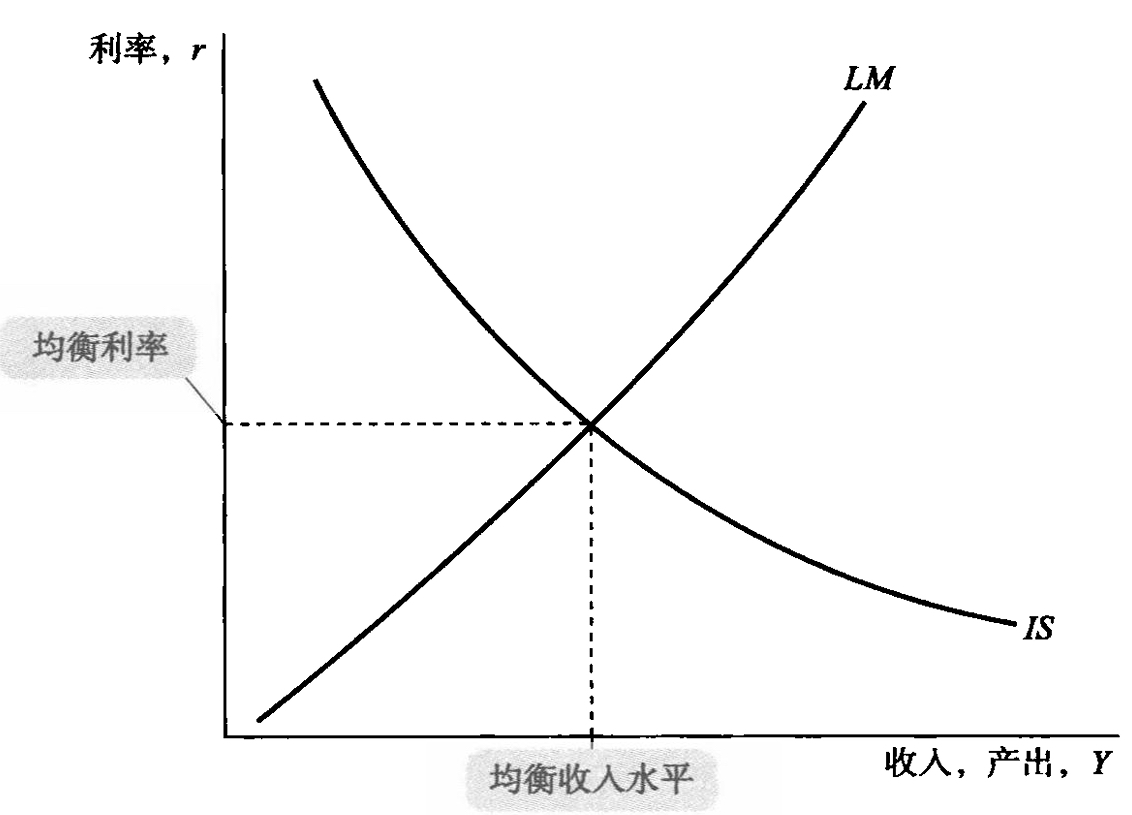
\includegraphics[width=0.5\textwidth]{/Users/lhr45678/Dropbox/hnu-macro-2021/IMG_0718.jpg}
\caption{IS-LM 曲线}
\label{fig:is-lm2}
\end{figure}

\paragraph{总结}

\begin{enumerate}
\item
  IS 曲线: 理论基础是凯恩斯交叉模型. 曲线向下倾斜,  因为更高的利率会降低投资,  进而降低总收入.
\item
  流动性偏好理论: 人们愿意持有货币,  是因为货币可以提供流动性. 实际货币余额需求 $L(Y, r)$ 和$Y$正相关, 和 $r$ 负相关.
\item
  LM 曲线: 理论基础是流动性偏好. 曲线向上倾斜, 因为更高的收入提高了实际货币余额需求,  进而提高了利率.
\item
  IS 曲线表示满足产品市场均衡的利率与收入,  LM
  曲线表示满足货币市场均衡的利率与收入,  其交点表示同时满足这两个市场均衡的利率与收入,  见图 \ref{fig:is-lm2}. 
\end{enumerate}

学习了 IS-LM 模型,  同学们就可以像宏观经济学家一样, 
自如地分析\textbf{货币政策和财政政策}的短期经济影响.
这部分内容我们留到之后再专门讨论.

%此外,  IS-LM 模型也是下一章推导总需求曲线的理论基础.
%这一部分的理论脉络见下图, 
%我们的终极目标是一个可用于描绘\textbf{短期内经济波动}的模型.
%
%\begin{figure}[h]
%\centering
%\includegraphics[width=0.9\textwidth]{~/Downloads/IMG_0719.jpg}
%\end{figure}

\paragraph{练习}
考虑三部门经济,  已知 $C=800+0.63Y$,  $I = 7500-20000r$, 
$L=0.1625Y-10000r$,  $G=7500$,  名义货币供给 $\bar{M} = 6000$,  价格水平 $\bar{P} = 1$.
(1) 推导IS曲线.
(2) 推导LM曲线.
(3) 计算均衡时的利率和投资水平.
(4) 当政府购买上升到 $8500$ 时,  计算私人投资的变化.
\hfill{(\textit{教材106页,  Q7})}

\end{document}